% wk 7 notes are incomplete
% lec 23
% wk 9
% expand upon Groups, Counting, Graphs

\documentclass{article}



% \usepackage{amsmath}
\usepackage{graphicx} \graphicspath{{./assets/}}
\usepackage{float} \restylefloat{table}
% \usepackage{amssymb}
% \usepackage{amsmath}
% \usepackage{amsthm}
\usepackage{multicol}
\usepackage{arydshln}
\usepackage[top=2cm,bottom=2cm,left=2cm,right=2cm]{geometry}
% \usepackage{mathtools}
\usepackage[super]{nth}

% \usepackage{amsmath,amssymb,amsfonts,amsthm,mathtools}
\usepackage[margin=15mm]{geometry}
\usepackage[dvipsnames]{xcolor}
\usepackage{graphicx}
\usepackage{tcolorbox}
\usepackage[final]{pdfpages}
\usepackage{gauss}
\usepackage{relsize}
\usepackage{etoolbox}
\usepackage[en-GB,showzone=false]{datetime2}
% \setlength\parindent{0pt}
\usepackage{parskip}

% From Toms preamble
\usepackage[framemethod=TikZ]{mdframed}
\usepackage{float} \restylefloat{table}
% \definecolor{peach}{RGB}{255,218,185} % Custom colours


\graphicspath{ {./} }

\allowdisplaybreaks

%-------------------------------------------- COMMANDS
\newcommand{\sidebyside}[2]{

      \noindent\begin{minipage}[t]{.5\linewidth}
            #1
      \end{minipage}%
      \noindent\begin{minipage}[t]{.5\linewidth}
            #2
      \end{minipage}
      
      }

\newcommand{\sidebysidebyside}[3]{
      
      \noindent\begin{minipage}[t]{.3\linewidth}
            #1
      \end{minipage}%
      \noindent\begin{minipage}[t]{.3\linewidth}
            #2
      \end{minipage}%
      \noindent\begin{minipage}[t]{.3\linewidth}
            #3
      \end{minipage}
      
      }

\newcommand{\diff}{\, \mathrm{d}}

\newcommand{\ddiff}[1]{\, \frac{\mathrm{d}}{\mathrm{d}  #1}}

\newcommand{\limtoinfinity}[1]{\lim_{#1 \to \infty}}

\newcommand{\limtoneginfinity}[1]{\lim_{#1 \to -\infty}}

\newcommand{\abs}[1]{\left| #1 \right|}

% \newcommand{\det}{\, \mathrm{det}}


\newcommand{\coversheet}[2]{
    \includepdf[pagecommand={
    \begin{tikzpicture}[remember picture, overlay]
        \node[inner sep=0pt,scale=0.5] (Signature) at (3,-20.75) {\includegraphics[width=.25\textwidth]{/home/jake/Uni/Signature/Signature.png}};
        \node[inner sep=0pt] (Date) at (5.3,-11.2) {\textsf{\today}};
        \node[inner sep=0pt] (Gav) at (11.8,-10.05) {\textsf{#1}};
        \node[inner sep=0pt] (Tut time) at (11.9,-11) {\textsf{#2}};
        \node[inner sep=0pt] (Date) at (14.55,-20.75) {\textsf{\today}};
    \end{tikzpicture}}]{Coversheet}
}

%augmented matrix line
\makeatletter
\patchcmd\g@matrix
 {\vbox\bgroup}
 {\vbox\bgroup\normalbaselines}% restore the standard base line skip
 {}{}
\makeatother


\newcommand{\mline}[1][0pt]{%
  \hspace{-\arraycolsep}%
  \ifdim#1>0pt
    \dimen0=\ht\strutbox \dimen2=\dimen0
    \advance\dimen0 #1\relax
    \ht\strutbox=\dimen0
  \fi
  \smash{\strut\vrule} % the `\vrule` is as high and deep as a strut
  % since assignments to \ht\strutbox are global, we restore the height
  \ifdim#1>0pt
    \ht\strutbox=\dimen2
  \fi
  \hspace{-\arraycolsep}%
}

% tikz if statement on by default

\newif\ifshowtikz
\showtikztrue

% \showtikzfalse   % <---- comment/uncomment that line
\ifshowtikz
\usepackage{tikz}
\usetikzlibrary{backgrounds}
\usetikzlibrary{arrows}
\usetikzlibrary{shapes,shapes.geometric,shapes.misc}

% this style is applied by default to any tikzpicture included via \tikzfig
\tikzstyle{tikzfig}=[baseline=-0.25em,scale=0.5]

% these are dummy properties used by TikZiT, but ignored by LaTex
\pgfkeys{/tikz/tikzit fill/.initial=0}
\pgfkeys{/tikz/tikzit draw/.initial=0}
\pgfkeys{/tikz/tikzit shape/.initial=0}
\pgfkeys{/tikz/tikzit category/.initial=0}

% standard layers used in .tikz files
\pgfdeclarelayer{edgelayer}
\pgfdeclarelayer{nodelayer}
\pgfsetlayers{background,edgelayer,nodelayer,main}

% style for blank nodes
\tikzstyle{none}=[inner sep=0mm]

% include a .tikz file
\newcommand{\tikzfig}[1]{%
{\tikzstyle{every picture}=[tikzfig]
\IfFileExists{./figures/#1.tikz}
  {\input{./figures/#1.tikz}}
  {%
    \IfFileExists{#1.tikz}
      {\input{#1.tikz}}
      {\tikz[baseline=-0.5em]{\node[draw=red,font=\color{red},fill=red!10!white] {\textit{#1}};}}%
  }}%
}

% the same as \tikzfig, but in a {center} environment
\newcommand{\ctikzfig}[1]{%
\begin{center}\rm
  \tikzfig{#1}
\end{center}}

% fix strange self-loops, which are PGF/TikZ default
\tikzstyle{every loop}=[]




\input{/home/jake/Uni/LaTeX files/tikzpaper/Standard.tikzstyles}
\else
\newcommand{\tikzfig}[1]{}
\newcommand{\ctikzfig}[1]{}
\fi 

% \renewcommand{\thesection}{\hspace{5pt} \arabic{section}.}

\newcommand{\mychapter}[2]{
    \setcounter{chapter}{#1}
    \setcounter{section}{0}
    \chapter*{#2}
    \addcontentsline{toc}{chapter}{#2}
}



% this stupid shit breaks my bracket colourer so I had to make a new command so I don't have miss matched colours
\newcommand{\rightopenleftclosed}[1]{\left[ \left. #1 \right) \right. } 
\newcommand{\leftopenrightclosed}[1]{\left( \left. #1 \right] \right. }

% \mdfsetup{skipabove=\topskip,skipbelow=\topskip}

% % THEOREM
% \newcounter{theo}[section] \setcounter{theo}{0}
% \renewcommand{\thetheo}{\arabic{section}.\arabic{theo}}
% \newenvironment{theorem}[1][]{%
% \refstepcounter{theo}%
% \ifstrempty{#1}%
% {\mdfsetup{%
% frametitle={%
% \tikz[baseline=(current bounding box.east),outer sep=0pt]
% \node[anchor=east,rectangle,fill=blue!20, rounded corners=0.8mm]
% {\strut Theorem~\thetheo};}}
% }%
% {\mdfsetup{%
% frametitle={%
% \tikz[baseline=(current bounding box.east), outer sep=0pt]
% \node[anchor=east,rectangle,fill=blue!20, rounded corners=0.8mm]
% {\strut Theorem~\thetheo:~#1};}}%
% }%
% \mdfsetup{innertopmargin=10pt,linecolor=blue!20,%
% linewidth=2pt,topline=true,%
% frametitleaboveskip=\dimexpr-\ht\strutbox\relax
% }
% \begin{mdframed}[]\relax%
% }{\end{mdframed}}

% THEOREM
\newenvironment{theorem}[1][]{%
\ifstrempty{#1}%
{\mdfsetup{%
frametitle={%
\tikz[baseline=(current bounding box.east),outer sep=0pt]
\node[anchor=east,rectangle,fill=blue!20, rounded corners=0.8mm]
{\strut Theorem};}}
}%
{\mdfsetup{%
frametitle={%
\tikz[baseline=(current bounding box.east),outer sep=0pt]
\node[anchor=east,rectangle,fill=blue!20, rounded corners=0.8mm]
{\strut Theorem:~#1};}}%
}%
\mdfsetup{innertopmargin=10pt,linecolor=blue!20,%
linewidth=2pt,topline=true,%
frametitleaboveskip=\dimexpr-\ht\strutbox\relax
}
\begin{mdframed}[]\relax%
}{\end{mdframed}}



% DEFINITION
\newcounter{defi}[section] \setcounter{defi}{0}
\renewcommand{\thedefi}{\arabic{section}.\arabic{defi}}
\newenvironment{definition}[1][]{%
\refstepcounter{defi}%
\ifstrempty{#1}%
{\mdfsetup{%
frametitle={%
\tikz[baseline=(current bounding box.east),outer sep=0pt]
\node[anchor=east,rectangle,fill=green!20, rounded corners=0.8mm]
{\strut Definition~\thedefi};}}
}%
{\mdfsetup{%
frametitle={%
\tikz[baseline=(current bounding box.east),outer sep=0pt]
\node[anchor=east,rectangle,fill=green!20, rounded corners=0.8mm]
{\strut Definition~\thedefi:~#1};}}%
}%
\mdfsetup{innertopmargin=10pt,linecolor=green!20,%
linewidth=2pt,topline=true,%
frametitleaboveskip=\dimexpr-\ht\strutbox\relax
}
\begin{mdframed}[]\relax%
}{\end{mdframed}}



% LEMMMA
\newcounter{lema}[section] \setcounter{lema}{0}
\renewcommand{\thelema}{\arabic{section}.\arabic{lema}}
\newenvironment{lemma}[1][]{%
\refstepcounter{lema}%
\ifstrempty{#1}%
{\mdfsetup{%
frametitle={%
\tikz[baseline=(current bounding box.east),outer sep=0pt]
\node[anchor=east,rectangle,fill=red!20, rounded corners=0.8mm]
{\strut Lemma~\thelema};}}
}%
{\mdfsetup{%
frametitle={%
\tikz[baseline=(current bounding box.east),outer sep=0pt]
\node[anchor=east,rectangle,fill=red!20, rounded corners=0.8mm]
{\strut Lemma~\thelema:~#1};}}%
}%
\mdfsetup{innertopmargin=10pt,linecolor=red!20,%
linewidth=2pt,topline=true,%
frametitleaboveskip=\dimexpr-\ht\strutbox\relax
}
\begin{mdframed}[]\relax%
}{\end{mdframed}}

% EXAMPLE
\newcounter{exam}[section] \setcounter{exam}{0}
\renewcommand{\theexam}{\arabic{section}.\arabic{exam}}
\newenvironment{example}[1][]{%
\refstepcounter{exam}%
\ifstrempty{#1}%
{\mdfsetup{%
frametitle={%
\tikz[baseline=(current bounding box.east),outer sep=0pt]
\node[anchor=east,rectangle,fill=orange!20, rounded corners=0.8mm]
{\strut Example~\theexam};}}
}%
{\mdfsetup{%
frametitle={%
\tikz[baseline=(current bounding box.east),outer sep=0pt]
\node[anchor=east,rectangle,fill=orange!20, rounded corners=0.8mm]
{\strut Example~\theexam:~#1};}}%
}%
\mdfsetup{innertopmargin=10pt,linecolor=orange!20,%
linewidth=2pt,topline=true,%
frametitleaboveskip=\dimexpr-\ht\strutbox\relax
}
\begin{mdframed}[]\relax%
}{\end{mdframed}}

% PROPOSITION
\newcounter{prop}[section] \setcounter{prop}{0}
\renewcommand{\theprop}{\arabic{section}.\arabic{prop}}
\newenvironment{proposition}[1][]{%
\refstepcounter{prop}%
\ifstrempty{#1}%
{\mdfsetup{%
frametitle={%
\tikz[baseline=(current bounding box.east),outer sep=0pt]
\node[anchor=east,rectangle,fill=orange!20, rounded corners=0.8mm]
{\strut Proposition~\theprop};}}
}%
{\mdfsetup{%
frametitle={%
\tikz[baseline=(current bounding box.east),outer sep=0pt]
\node[anchor=east,rectangle,fill=orange!20, rounded corners=0.8mm]
{\strut Proposition~\theprop:~#1};}}%
}%
\mdfsetup{innertopmargin=10pt,linecolor=orange!20,%
linewidth=2pt,topline=true,%
frametitleaboveskip=\dimexpr-\ht\strutbox\relax
}
\begin{mdframed}[]\relax%
}{\end{mdframed}}

% CLAIM
\newenvironment{claim}[1][]{%
\ifstrempty{#1}%
{\mdfsetup{%
frametitle={%
\tikz[baseline=(current bounding box.east),outer sep=0pt]
\node[anchor=east,rectangle,fill=Lavender!50, rounded corners=0.8mm]
{\strut Claim};}}
}%
{\mdfsetup{%
frametitle={%
\tikz[baseline=(current bounding box.east),outer sep=0pt]
\node[anchor=east,rectangle,fill=Lavender!50, rounded corners=0.8mm]
{\strut Claim:~#1};}}%
}%
\mdfsetup{innertopmargin=10pt,linecolor=Lavender!50,%
linewidth=2pt,topline=true,%
frametitleaboveskip=\dimexpr-\ht\strutbox\relax
}
\begin{mdframed}[]\relax%
}{\end{mdframed}}


% NOTE
\newenvironment{note}%
{\begin{quote}\textbf{Note}:}%
{\end{quote}}


% OBSERVATION
\newenvironment{observation}%
{\begin{quote}\textbf{Obs}:}%
{\end{quote}}

% TOOL
\newenvironment{tool}%
{\begin{quote}\textbf{Tool}:}%
{\end{quote}}

% FACT
\newenvironment{fact}%
{\begin{quote}\textbf{Fact}:}%
{\end{quote}}

% IDEA
\newenvironment{idea}%
{\begin{quote}\textbf{Idea}:}%
{\end{quote}}

% Corollary
\newenvironment{corollary}%
{\begin{quote}\textbf{Corollary}:}%
{\end{quote}}

% Question
\newenvironment{question}%
{\begin{quote}\textbf{Q}:}%
{\end{quote}}

% % Remark
% \newenvironment{remark}%
% {\begin{quote}\textbf{Remark}:}%
% {\end{quote}}

% REMARK
\newenvironment{remark}[1][]{%
\ifstrempty{#1}%
{\mdfsetup{%
frametitle={%
\tikz[baseline=(current bounding box.east),outer sep=0pt]
\node[anchor=east,rectangle,fill=NavyBlue!20, rounded corners=0.8mm]
{\strut Remark};}}
}%
{\mdfsetup{%
frametitle={%
\tikz[baseline=(current bounding box.east),outer sep=0pt]
\node[anchor=east,rectangle,fill=NavyBlue!20, rounded corners=0.8mm]
{\strut Remark:~#1};}}%
}%
\mdfsetup{innertopmargin=10pt,linecolor=NavyBlue!20,%
linewidth=2pt,topline=true,%
frametitleaboveskip=\dimexpr-\ht\strutbox\relax
}
\begin{mdframed}[]\relax%
}{\end{mdframed}}

% Notation
\newenvironment{notation}%
{\begin{quote}\textbf{Notation}:}%
{\end{quote}}


%shits gotta come last ffs
\usepackage{hyperref}
\hypersetup{pdfauthor={Jake Moss}, pdfkeywords={s46409665 - jake.moss@uqconnect.edu.au}}

\usepackage{amsmath,amssymb,amsfonts,amsthm,mathtools}
% \usepackage[margin=15mm]{geometry}
\usepackage[dvipsnames]{xcolor}
% \usepackage{graphicx}
\usepackage{tcolorbox}
\usepackage[final]{pdfpages}
% \usepackage{gauss}
\usepackage{relsize}
\usepackage{etoolbox}
% \usepackage[en-GB,showzone=false]{datetime2}
% \setlength\parindent{0pt}
\usepackage{parskip}

% From Toms preamble
\usepackage[framemethod=TikZ]{mdframed}
\usepackage{float} \restylefloat{table}
% \definecolor{peach}{RGB}{255,218,185} % Custom colours

\usepackage{hyperref}

\newcommand{\ts}{\textsuperscript}



\DeclarePairedDelimiter\ceil{\lceil}{\rceil}
\DeclarePairedDelimiter\floor{\lfloor}{\rfloor}

\setcounter{tocdepth}{2}


\setlength{\dashlinedash}{1pt}
\setlength{\dashlinegap}{2pt}
\setlength{\arrayrulewidth}{0.2pt}


\theoremstyle{definition}
% \newtheorem*{definition}{Definition}
% \newtheorem*{example}{Examples}
% \newtheorem*{theorm}{Theorm}
\newtheorem*{remark}{Remark}
\newtheorem*{observation}{Observation}
\newtheorem*{proposition}{Proposition}


% THEOREM
\newenvironment{theorm}[1][]{%
\vspace{3mm}
\ifstrempty{#1}%
{\mdfsetup{%
frametitle={%
\tikz[baseline=(current bounding box.east),outer sep=0pt]
\node[anchor=east,rectangle,fill=blue!20, rounded corners=0.8mm]
{\strut Theorem};}}
}%
{\mdfsetup{%
frametitle={%
\tikz[baseline=(current bounding box.east),outer sep=0pt]
\node[anchor=east,rectangle,fill=blue!20, rounded corners=0.8mm]
{\strut Theorem:~#1};}}%
}%
\mdfsetup{innertopmargin=10pt,linecolor=blue!20,%
linewidth=2pt,topline=true,%
frametitleaboveskip=\dimexpr-\ht\strutbox\relax
}
\begin{mdframed}[]\relax%
}{\end{mdframed}}


% definition
\newenvironment{definition}[1][]{%
\vspace{3mm}
\ifstrempty{#1}%
{\mdfsetup{%
frametitle={%
\tikz[baseline=(current bounding box.east),outer sep=0pt]
\node[anchor=east,rectangle,fill=green!20, rounded corners=0.8mm]
{\strut Definition};}}
}%
{\mdfsetup{%
frametitle={%
\tikz[baseline=(current bounding box.east),outer sep=0pt]
\node[anchor=east,rectangle,fill=green!20, rounded corners=0.8mm]
{\strut Definition:~#1};}}%
}%
\mdfsetup{innertopmargin=10pt,linecolor=green!20,%
linewidth=2pt,topline=true,%
frametitleaboveskip=\dimexpr-\ht\strutbox\relax
}
\begin{mdframed}[]\relax%
}{\end{mdframed}}


% example
\newenvironment{example}[1][]{%
\vspace{3mm}
\ifstrempty{#1}%
{\mdfsetup{%
frametitle={%
\tikz[baseline=(current bounding box.east),outer sep=0pt]
\node[anchor=east,rectangle,fill=orange!20, rounded corners=0.8mm]
{\strut Example};}}
}%
{\mdfsetup{%
frametitle={%
\tikz[baseline=(current bounding box.east),outer sep=0pt]
\node[anchor=east,rectangle,fill=orange!20, rounded corners=0.8mm]
{\strut Example:~#1};}}%
}%
\mdfsetup{innertopmargin=10pt,linecolor=orange!20,%
linewidth=2pt,topline=true,%
frametitleaboveskip=\dimexpr-\ht\strutbox\relax
}
\begin{mdframed}[]\relax%
}{\end{mdframed}}

% \newenvironment{example}{
% \begin{tabular}{:p{0.9\textwidth}:}
%     \hdashline\\\textbf{Ex.}
%     }
%     {
%     \\\\\hdashline
%     \end{tabular}
% }

\setlength{\parindent}{0pt}

\author{Tom Stephen, Edited by Ben Kruger, Stylised by Jake Moss}
\title{\vspace{-15mm} MATH1061 - Course Notes}

\begin{document}

\maketitle 
\tableofcontents

\newpage
\section{Logic}
\subsection{Logical Form}
\begin{definition}A \underline{statement} or \underline{proposition} is a sentence that is either true or false, but not both.\end{definition}

\begin{example}
Statements: \begin{itemize}
    \item The number 5 is even
    \item $\pi > 3$
    \item Leonhard Euler was born in 1707
\end{itemize}

Not statements: \begin{itemize}
    \item How are you?
    \item Stop!
    \item She likes maths. (we do not know who she is)
    \item $x^2 = 2x - 1$ (we do not know the value of $x$)
\end{itemize}
\end{example}

\begin{definition}Let $p$ be a statement. The \underline{negation} of $p$ is denoted as $\sim p$ or $\neg p$ (read as ``not $p$'').$$\begin{array}{|c|c|}
p & \sim p \\
\hline
T & F \\
F & T
\end{array}$$
\end{definition}


Let $p$ and $q$ be statements.

\begin{definition}The \underline{conjunction} of $p$ and $q$ is denoted $p \land q$ (read as ``$p$ and $q$'')$$\begin{array}{|c c|c|}
p & q & p\land q \\
\hline
T & T & T \\
T & F & F \\
F & T & F \\
F & F & F
\end{array}$$\end{definition}


\newpage
\begin{definition}The \underline{disjuction} of $p$ and $q$ is denoted $p \lor q$ (read as ``$p$ or $q$'')$$\begin{array}{|c c|c|}
p & q & p\lor q \\
\hline
T & T & T \\
T & F & T \\
F & T & T \\
F & F & F
\end{array}$$\end{definition}



Think of $p$,$q$,$r$ as \underline{statement variables}.

\begin{definition}
    A \underline{statement form} is made up from statement variables ($p,q,r$) and the symbols $\sim , \land, \lor$ with unambiguous parentheses.
\end{definition}

\begin{example}
    $$P = \sim \left(p\lor r\right)\land\left(\sim r\right)$$ is a statement form. How many rows will a truth table for $P$ need? We realise we have 3 statement variables, so we will need $2^3 = 8$ rows.
\end{example}


\subsection{Logical Equivalence}
\begin{definition}
    Two statement forms $P$ and $Q$ are \underline{logically equivalent}, denoted $P\equiv Q$, if they have identical truth values for every possible combination of truth values for their statement variables.
\end{definition}

\begin{example}
    $$\sim\left(\sim p\right) \equiv p$$
\end{example}

\begin{multicols}{2}
\subsubsection{Demorgan's Law}
$$\sim\left(p\land q\right) \equiv \sim p \lor \sim q$$
$$\sim\left(p\lor q\right) \equiv \sim p \land \sim q$$

\subsubsection{Commutativity}
$$p\land q \equiv q \land p$$
$$p\lor q \equiv q \lor p$$

\subsubsection{Associativity}
$$p\land \left(q\land r\right) \equiv \left(p\land q\right)\land r$$
$$p\lor \left(q\lor r\right) \equiv \left(p\lor q\right)\lor r$$

\subsubsection{Distributive Laws}
$$p\land \left(q\lor r\right) \equiv \left(p\land q\right) \lor \left(p\land r\right)$$
$$p\lor \left(q\land r\right) \equiv \left(p\lor q\right) \land \left(p\lor r\right)$$

\subsubsection{Double Negative}
$$\sim\left(\sim p\right) \equiv p$$

\subsubsection{Idempotent Laws}
$$p\land p \equiv p$$
$$p\lor p\equiv p$$

\subsubsection{Absorption Laws}
$$p\lor \left(p\land q\right)\equiv p$$
$$p\land \left(p\lor q\right)\equiv p$$
\end{multicols}


\subsubsection{Tautolgy and Contradiction}
\begin{definition}
    A \underline{tautolgy} is a statement form which always takes the truth value \emph{true} for all possible truth values of its variables.
\end{definition}

\begin{example}
    $$\begin{array}{|c c|c|}
    p & \sim p & p\lor \sim p\\
    \hline
    T & F & T\\
    F & T & T
    \end{array}$$
\end{example}

\begin{definition}
    A \underline{contradiction} is a statement form which always takes the truth value \emph{false} for all possible truth values of its variables.
\end{definition}

\begin{example}
    $$\begin{array}{|c c|c|}
    p & \sim p & p\land \sim p\\
    \hline
    T & F & F\\
    F & T & F
    \end{array}$$
\end{example}

\begin{multicols}{2}
\subsubsection{Identity Laws}
$$p\land \left(\text{tautolgy}\right) \equiv p$$
$$p\lor \left(\text{contradiction}\right) \equiv p$$

\subsubsection{Universal Bound Law}
$$p\lor \left(\text{tautolgy}\right) \equiv \left(\text{tautolgy}\right)$$
$$p\land \left(\text{contradiction}\right) \equiv \left(\text{contradiction}\right)$$

\subsubsection{Negation Laws}
$$p\lor \sim p \equiv \text{tautolgy}$$
$$p\land \sim p \equiv \text{contradiction}$$

\subsubsection{Negations}
$$\sim \left(\text{tautolgy}\right) \equiv \text{contradiction}$$
$$\sim \left(\text{contradiction}\right) \equiv \text{tautolgy}$$
\end{multicols}

\subsection{Conditional Statements}
\begin{definition}
    Let $p$ and $q$ be statement variables. The \underline{conditional} from $p$ to $q$, denoted $p\rightarrow q$ (read as ``$p$ implies $q$'' or ``if $p$ then $q$''), is defined by the following truth table:
    $$\begin{array}{|c c|c|}
    p & q & p\rightarrow q\\
    \hline
    T & T & T\\
    T & F & F\\
    F & T & T\\
    F & F & T
    \end{array}$$
\end{definition}

\subsubsection{Expressing the Conditional with Logical Connectives}
$$p\rightarrow q \equiv \sim p \lor q$$

\subsubsection{Contrapositive}
\begin{definition}
    The \underline{contrapositive} of $p\rightarrow q$ is $\sim q \rightarrow \sim p$. These are logically equivalent.
\end{definition}

\subsubsection{Negation of $p\rightarrow q$}
$$\sim\left(p\rightarrow q\right) \equiv p\land \sim q$$

\subsubsection{Biconditional Statements}
\begin{definition}
    Let $p$ and $q$ be statement variables. The \underline{biconditional} of $p$ and $q$, denoted $p\leftrightarrow q$ (read as ``$p$ if and only if $q$''), is defined by the following truth table:
    $$\begin{array}{|c c|c|}
    p & q & p\leftrightarrow q\\
    \hline
    T & T & T\\
    T & F & F\\
    F & T & F\\
    F & F & T
    \end{array}$$
\end{definition}

\subsection{Arguments}
\begin{definition}
    Given a collection of statements $p_1,p_2,\dots,p_n$ (called \underline{premises}) and another statement $q$ (called the \underline{conclusion}), an \underline{argument} is the assertion that the conjunction of the premises implies the conclusion. Symbolically, this is represented as \begin{align*}p_1 \\ p_2 \\ \vdots \\ p_3 \\ \therefore q\end{align*}
\end{definition}

\begin{definition}
    An argument is \underline{valid} if whenever all of the premises are true, the conclusion is also true.

    Thus, an argument is valid if $$\left(p_1\land p_2 \land \dots \land p_n\right)\rightarrow q$$ is a tautolgy.
\end{definition}

\subsubsection{Rules of Inference}
\begin{multicols}{2}
Modus Ponens
\begin{align*}
    &p\rightarrow q \\
    &p \\
    \therefore q
\end{align*}

Modus Tollens
\begin{align*}
    p\rightarrow q \\
    \sim q\\
    \therefore \sim p
\end{align*}

Generalisation
\begin{align*}
    &p \qquad\qquad q\\
    &\therefore p\lor q \quad\therefore p\lor q
\end{align*}

Specialisation
\begin{align*}
    &p\land q\qquad p\land q \\
    &\therefore p \qquad \therefore q
\end{align*}

Conjunction
\begin{align*}
    &p\\
    &q\\
    &\therefore p\land q
\end{align*}

Elimination
\begin{align*}
    &p\lor q \quad p\lor q\\
    &\sim q \qquad \sim p\\
    &\therefore p \qquad \therefore q
\end{align*}

Transitivity
\begin{align*}
    p\rightarrow q \\
    q\rightarrow r \\
    \therefore p\rightarrow r
\end{align*}

Proof by Division into Cases
\begin{align*}
    &p\lor q \\
    &p\rightarrow r\\
    &q\rightarrow r\\
    &\therefore r
\end{align*}

Contradiction rule
\begin{align*}
    &\sim p\rightarrow \left(\text{contradiction}\right)\\
    &\therefore p
\end{align*}
\end{multicols}

\subsection{Quantified Statements}
\begin{definition}
    A \underline{predicate} is a sentence that contains finitely many variables, and which becomes a statement if the variables are given specific values. The \underline{domain} of each variable in a predicate is the set of all possible values that may be assigned to it.
\end{definition}

\begin{definition}
    The \underline{truth set} of a predicate $P(x)$ is the set of all values in the domain that, when assigned to $x$, make $P(x)$ a true statement.
\end{definition}

\begin{example}
    Let $P(x)$ be the predicate ``$x$ divides 5'' with the set of integers as the domain of $x$. The truth set of $P(x)$ is $\{-5,-1,1,5\}$
\end{example}

\subsubsection{Common Domains}
\begin{table}[H]
\begin{tabular}{|l|l|l|}
\hline
Domain & Symbol & Example \\
\hline
Integers & $\mathbb{Z}$ & $\{\dots,-3,-2,-1,0,1,2,3,\dots\}$ \\
Positive Integers & $\mathbb{Z}^+$ & $\{1,2,3,\dots\}$ \\
Non-negative Integers & $\mathbb{Z}^\text{nonneg} \text{ or } \mathbb{Z}^{\geq 0}$ & $\{0,1,2,3,\dots\}$ \\
Natural Numbers & $\mathbb{N}$ & $\{1,2,3,\dots\}$ \\
Rational Numbers & $\mathbb{Q}$ & $\{\frac{a}{b} | a,b\in\mathbb Z \land b\neq 0\}$ \\
Real Numbers & $\mathbb{R}$ & the entire number line \\
\hline
\end{tabular}
\end{table}

\begin{definition}
    The Universal Quantifier: The symbol $\forall$ denotes ``for all'' (or ``for each'' or ``for every'') and is called the \underline{universal quantifier}. Let $Q(x)$ be a predicate and $D$ be the domain of $x$. The \underline{universal statement} $$\forall x\in D, Q(x)$$ is true if and only if $Q(x)$ is true for every $x$ in $D$. It is false if and only if $Q(x)$ is false for at least one $x$ in $D$.
\end{definition}

\begin{definition}
    The Existential Quantifier: The symbol $\exists$ denotes ``there exists'' (or ``there is'' or ``there are'') and is called the \underline{existential quantifier}. Let $Q(x)$ be a predicate and $D$ be the domain of $x$. The \underline{existential statement} $$\exists x\in D \text{ such that } Q(x)$$ is true if and only if $Q(x)$ is true for at least one $x$ in $D$. It is false if $Q(x)$ is false for every $x$ in $D$.
\end{definition}

\subsubsection{Universal Conditional Statements}
One of the most important statement forms in mathematics is $$\forall x \in D \text{ if } P(x) \text{ then } Q(x)$$ or equivalently, $$\forall x\in D, \left(P(x)\rightarrow Q(x)\right)$$

\subsubsection{Negation}
Recall universal statement $$\forall x\in D, Q(x)$$ The negation of this statement is logically equivalent to $$\exists x\in D \text{ such that } \sim Q(x)$$

Recall existential statement $$\exists x\in D \text{ such that } R(x)$$ The negation of this statement is logically equivalent to $$\forall x\in D, \sim R(x)$$

Recall universal conditional statement $$\forall x\in D \text{ if } P(x) \text{ then } Q(x)$$ The negation of this statement is logically equivalent to $$\exists x\in D \text{ such that } \sim\left(P(x)\rightarrow Q(x)\right)$$ which is $$\exists x\in D \text{ such that } P(x)\land\sim Q(x)$$

% \begin{multicols}{2}
% \end{multicols}
\section{Number Theory}
\subsection{Modulo Arithmetic}
\subsubsection{Floor and Ceiling}
\begin{definition}
	Given any $x\in\mathbb R$, the floor of $x$, denoted $\floor{x}$, is the unique integer $n$ such that $n \leq x < n + 1$

	Given any $x\in\mathbb R$, the ceiling of $x$, denoted $\ceil{x}$, is the unique integer $n$ such that $n-1 < x \leq n$
\end{definition}

\subsection{Euclidean Algorithm}
\begin{definition}
    For integers $a,b\in\mathbb Z$, not both zero, the \underline{greatest common divisor} of $a$ and $b$, denoted $\text{gcd}\left(a,b\right)$, is the integer $d$ which satisfies the following two properties:
    \begin{itemize}
        \item $d|a$ and $d|b$
        \item for all $c\in\mathbb Z$, if $c|a$ and $c|b$, then $c\geq d$
    \end{itemize}
    Thus $d$ is the largest integer for which $d|a$ and $d|b$
\end{definition}

If $\text{gcd}\left(a,b\right) = 1$ then $a$ and $b$ have no common factors other than $\pm 1$ and we call $a$ and $b$ co-prime or relatively prime.

\textbf{Fact}: If $a$ and $b$ are integers with $b\neq 0$ and if $q$ and $r$ are integers such that $$a = bq + r$$ then $$\text{gcd}\left(a,b\right) = \text{gcd}\left(b,r\right)$$

\begin{definition}
    The Euclidean Algorithm: to find $\text{gcd}\left(a,b\right)$ where $a,b\in\mathbb Z$ and $a\geq b>0$,
    \begin{itemize}
        \item write $a=bq+r$, as in the quotient-remainder theorem
        \item if $r=0$, then terminate with $\text{gcd}\left(a,b\right)=b$
        \item otherwise replace $\left(a,b\right)$ with $\left(b,r\right)$ and repeat
    \end{itemize}
\end{definition}

\begin{definition}
    For non-zero integers $a,b\in\mathbb Z$, the \underline{lowest common multiple} of $a$ and $b$ is the smallest positive integer $n$ for which $a|n$ and $b|n$. We write this as $\text{lcm}\left(a,b\right)$
\end{definition}

\textbf{Fact}: suppose $a,b\in\mathbb{Z}$ where $a\geq b > 0$. Then $$\text{gcd}\left(a,b\right)\cdot\text{lcm}\left(a,b\right) = a\cdot b$$

\newpage
\subsection{Sequences}
\begin{definition}
    A \underline{sequence} is an ordered list of elements. It can be infinite or finite. Each individual element is called a \underline{term}. We often denote the terms of sequences by lower case letters with subscripts.
\end{definition}

An \underline{explicit formula} or \underline{general formula} for a sequence is a rule showing how the value of a general term $a_k$ depends upon $k$.

\begin{example}
$$1,2,3,4,5,\dots$$
The listed terms $a_0, a_1, a_2, \dots$ follow a pattern, where $a_k = 2^k$.

Different notations are used to denote such a sequence, such as $$\left\{2^k\right\}_{k\geq 0}\,\text{or}\,\left\{2^k\right\}^\infty_{k=0}\,\text{or}\,\left(2^k\right)_{k\geq 0}\,\text{or}\,\left(2^k\right)^\infty_{k=0}$$
\end{example}

\begin{example}
    Write the first 5 terms of $\left\{\frac{\left(-1\right)^n}{n}\right\}_{n\geq 1}$

    $$a_1 = -1,\, a_2 = \frac12,\, a_3 = -\frac13,\, a_4 = \frac14,\, a_5 = -\frac15$$
\end{example}

\begin{definition}
    An \underline{alternating sequence} is a sequence in which the terms alternate between positive and negative, such as the previous example.
\end{definition}

It is often useful to find a general term from initial terms.

\begin{example}
    Find a general formula for a sequence that has the following initial terms

    $$2,\, \frac34,\, \frac49,\, \frac{5}{16},\, \frac{6}{25},\, \frac{7}{36},\dots$$

    Let $a_n$ denote the general term and suppose the initial term is $a_1$. Observe that the denominator of each term is a perfect square and we can rewrite the terms as

    $$\frac{1+1}{1^2},\, \frac{2+1}{2^2},\, \frac{3+1}{3^2},\, \frac{4+1}{4^2},\, \frac{5+1}{5^2},\, \frac{6+1}{6^2},\dots$$

    Thus, the general term $$a_n = \frac{n+1}{n^2}$$ or, the sequence $\left\{\frac{n+1}{n^2}\right\}_{n\geq 1}$ has the given initial terms.
\end{example}

\subsection{Summation Notation}
We use greek capital Sigma $\Sigma$ to indicate a sum. If $m,n\in\mathbb Z$ and $m\leq n$, then $$\sum_{i=m}^n a_i = a_m + a_{m+1} + \dots + a_{n-1} + a_n$$

\subsection{Dummy Variable}
\begin{example}
    The variable $i$ in $\sum a_i$ is a \underline{dummy variable}. You can use any letter here, as long as it does not have another meaning.
\end{example}

\subsection{Product Notation}
We use greek capital Pi $\Pi$ to indicate a product. If $m,n\in\mathbb Z$ and $m\leq n$, then $$\prod_{i=m}^n a_i = a_m\cdot a_{m+1}\cdot\dots\cdot a_{n-1}\cdot a_n$$

\subsection{Factorial}
For $n\in\mathbb Z^+$, we define $n!$ (read ``$n$ factorial'') to be $$n! = n(n-1)(n-2)\cdot\dots\cdot 3\cdot 2\cdot 1 = \prod_{i=1}^n$$ also, $0!=1$

\subsection{Properties of Summation and Product Notation}
If $a_m,\, a_{m+1},\, a_{m+2},\,\dots$ and $b_m,\, b_{m+1},\, b_{m+2},\,\dots$ are sequences of real numbers, and $c$ is any real number, then, for any integer $n\geq m$, the following hold.

\begin{enumerate}
    \item $\displaystyle\sum_{i=m}^n a_i \pm \sum_{i=m}^n b_1 = \sum_{i=m}^n a_i \pm b_i$
    \item $\displaystyle\sum_{i=m}^n ca_i = c\sum_{i=m}^n a_i$
    \item $\displaystyle\left(\prod_{i=m}^n a_i\right)\left(\prod_{i=m}^n b_1\right) = \prod_{i=m}^n a_ib_i$
\end{enumerate}

\newpage
\subsection{Mathematical Induction}
\begin{definition}
    The Principle of Mathematical Induction.

    Let $P(n)$ be a predicate that is defined for every integer $n\geq a$, where $a$ is some fixed integer. Suppose \begin{enumerate}
        \item $P(a)$ is true.
        \item For every integer $k\geq a$, $P(k)\rightarrow P(k+1)$
    \end{enumerate}
    Then $P(n)$ is true for every integer $n\geq a$
\end{definition}

\subsubsection{Strong Mathematical Induction}
\begin{definition}
	The Principle of Strong Mathematical Induction.

	Let $P(n)$ be a predicate that is defined for every integer $n\geq a$, where $a$ is some fixed integer, and let $b$ be an integer where $b\geq a$. Suppose:
	\begin{itemize}
		\item \emph{Base step}: $P(a),\,P(a+1),\,\dots,\,P(b)$ are all true
		\item \emph{Inductive Step}: For every integer $x \geq b$, if $P(a), \, P(a + 1),\,\dots,\, P(k)$ are all true, then $P(k+1)$ is true.
	\end{itemize}
	The $P(n)$ is true for every integer $n\geq a$.
\end{definition}


Prove that for every integer $n \geq 8$, we can form $n$ cent postage using only 3c and/or 5c stamps.

Before starting a proof, we observe:
\begin{align*}
	8 &= 5 + 3 \rightarrow 11 = (5 + 3) + 3 \\
	9 &= 3 + 3 + 3 \rightarrow 12 = (3 + 3 + 3) + 3 \\
	10 &= 5 + 5 \rightarrow 13 = (5+5)+3
\end{align*}
We can now use this idea in a formal proof.
\begin{proof}
	Let $P(n)$ be the predicate ``$n$ cent postage can be formed using only 3c and/or 5c stamps''

	\emph{Basis Step}: We can prove $P(8),\,P(9),\,P(10)$ direction, since
	\begin{align*}
		8 &= 5 + 3 \\
		9 &= 3 + 3 + 3 \\
		10 &= 5 + 5
	\end{align*}

	\emph{Inductive Hypothesis}: Suppose that for some integer $k \geq 10$, $P(8),\,\dots,\,P(k)$ are all true. We will use this to prove $P(k+1)$.

	Since $k\geq 10$, we have $k - 2 \geq 8$. Thus, by the Inductive Hypothesis, we can form $(k-2)c$ using 3c and 5c stamps. Now we can add 1 more 3c stamp to make $(k+1)c$ postage and so $P(k+1)$ is true.

	Therefore, by strong induction, it follows that $P(n)$ is true for every integer $n\geq 8$.
\end{proof}
\newpage
\subsubsection{Well Ordering Principle}
\begin{definition}
	The \emph{Well Ordering Principle} for the integers.

	If $S$ is a non-empty set of integers, all of which are greater than some fixed integer, then $S$ has a least element.
\end{definition}

\section{Recursive Definitions}
\begin{example}
    The sequence $$1,\,1,\,2,\,3,\,5,\,8,\,13,\,21,\,34,\,55,\,\dots$$ is called the \underline{Fibonacci Sequence}
\end{example}

\begin{definition}
    A \underline{recurrence relation} for a sequence $a_0,a_1,a_2,\dots$ is a formula that relates each term $a_k$ to some of its predecessors $a_{k-1},\dots,a_{k-i}$ where $i\in\mathbb Z$ and $k-i \geq 0$

    The \underline{initial conditions} for such a recurrence relation specify the values of some of the initial terms.
\end{definition}

\begin{example}
The Fibonacci sequence is defined recursively by $$F_0 = 1,\, F_1 = 1,\,\text{and}\,F_n = F_{n-1} + F_{n-2}$$
\end{example}

\subsection{Ways to Define Sequences}
A sequence can be defined
\begin{itemize}
    \item \emph{informally}, by listing the first few terms of the sequence until the pattern becomes obvious
    \item \emph{with a general formula}, by stating how a term $a_n$ depends on $n$ and stating where it starts
    \item \emph{recursively}, by giving a recurrence relation relating terms in the sequence to earlier ones and also some initial conditions
\end{itemize}

\subsection{Showing a Sequence Satisfies a Recurrence Relation}
\begin{example}
Show that the sequence $$a_k = 3\cdot 2^k,\,\text{for }k\geq 0$$ satisfies the recurrence relation $$a_n = 2a_{n-1},\,\text{for }n\geq 1$$

The sequence is $\displaystyle \left\{3\cdot 2^k\right\}_{k\geq 0} = 3,\,6,\,12,\,24,\,48,\,\dots$

For every integer $n\geq 1$ we have $a_n = 3\cdot 2^n$ and $a_{n-1} = 3\cdot 2^{n-1}$

Hence, $$a_n = 3\cdot 2^n = 3\cdot 2\cdot 2^{n-1} = 2 (3\cdot 2^{n-1}) = 2 a_{n-1}$$
\end{example}

\subsection{Generalised}
We have seen that sequences of numbers can be defined recursively. Many other objects can be defined recursively as well, such as: sets, sums, products and function.

A recursive definition for a set of objects requires three things:
\begin{enumerate}
    \item BASE: a statement that a certain object belongs in the set
    \item RECURSION: a collection of rules showing how to form new objects for the set from existing ones in the set
    \item RESTRICTION: a statement that no objects belong to the set other than those arising from steps 1 and 2
\end{enumerate}

\begin{example}
    Consider the set of all \underline{valid bracketings}. Every left bracket ( is matched with a right bracket ) and at every stage, reading left to right, there are at least as many left brackets as right brackets.
    $$(())()\text{ is valid}$$
    $$()()()\text{ is valid}$$
    $$())(()\text{ is invalid}$$

    \underline{Recursive definition of the set of valid brakcetings}
    \begin{enumerate}
        \item Base: an empty expression with no brackets is valid
        \item Recursion: \begin{enumerate}
            \item if B is valid, the (B) is also valid
            \item if B and C are valid, then BC is also valid
        \end{enumerate}
        \item Restriction: Any expression not derived from the rules above is not valid
    \end{enumerate}
\end{example}

\begin{definition}
    Arithmetic Sequences are defined as such:
    \[a_k = a_{k-1} + d \qquad a_n = a_0 +dn\]
    Geometric Sequences are defined as such:
    \[a_k = r\cdot a_{k-1} \qquad a_n = a_0\cdot r^n\]
\end{definition}


\section{Functions}
\subsection{One-to-one}
\begin{definition}
    Let $f$ be a function from a set $X$ to a set $Y$. The function $f$ is \underline{one-to-one} (or \underline{injective}) if and only if for all elements $x_1$ and $x_2$ in $X$, $$\text{if } f(x_1) = f(x_2),\,\text{then } x_1 = x_2$$
    Or, equivalently, for all elements $x_1$ and $x_2$ in $X$, $$\text{if } x_1 \neq x_2,\,\text{then } f(x_1) \neq f(x_2)$$

    A function $f: X\rightarrow Y$ is \underline{not one-to-one} if and only if there exist some $x_1$ and $x_2$ in $X$ such that $f(x_1) = f(x_2)$ and $x_1 \neq x_2$
\end{definition}

\begin{enumerate}
\item To prove a function $f: X\rightarrow Y$ is one-to-one, we typically use a direct proof: \begin{enumerate}
    \item suppose $x_1$ and $x_2$ are element of $X$, and $f(x_1) = f(x_2)$
    \item show that $x_1 = x_2$
\end{enumerate}

\item To prove that a function $f: X\rightarrow Y$ is not one-to-one, we typically find elements $x_1$ and $x_2$ in $X$ such that $f(x_1) = f(x_2)$ but $x_1 \neq x_2$
\end{enumerate}

\begin{example}
    Let $f: \mathbb R \rightarrow \mathbb R$ be defined by $f(x) = x^2$. Is $f$ one-to-one?

    Proof that $f$ is not one-to-one:
    \begin{proof}
        Take $x_1 = 2$ and $x_2 = -2$

        Since $f(2) = 4$ and $f(-2) = 4$, we have found different elements of the domain with the same image. Thus $f$ is not one-to-one.
    \end{proof}
\end{example}

\subsection{Onto}
\begin{definition}
    Let $f$ be a function from a set $X$ to a set $Y$. The function $f$ is \underline{onto} (or \underline{surjective}) if and only if given any element $y\in Y$, it is possible to find an element $x\in X$ with the property that $y = f(x)$.

    Equivalently, $f:X\rightarrow Y$ is onto if and only if $\forall y\in Y,\,\exists x\in X$ such that $f(x) = y$

    A function $f:X\rightarrow Y$ is \underline{not onto} if and only if there exists some $y\in Y$ such that for all $x\in X$, $f(x)\neq y$.
\end{definition}

\begin{itemize}
    \item To prove that a function $f: X\rightarrow Y$ is onto, we usually \begin{itemize}
        \item suppose that $y\in Y$
        \item construct an element $x$ of $X$ with $f(x) = y$
    \end{itemize}
    \item To prove that a function $f: X\rightarrow Y$ is not onto, we usually \begin{itemize}
        \item find an element $y\in Y$ such that $y \neq f(x)$ for any $x\in X$
    \end{itemize}
\end{itemize}

\newpage
\subsection{Inverse}
\begin{theorm}
    Suppose some function \(f: X\to Y\) is a bijection. Then, \[\exists f^{-1}: Y\to X\]
    That is defined,\\
    Given any \(y\in Y\), \(f^{-1}(y) = x\) for some unique element \(x\in X\) such that \(f(x) = y\). 
\end{theorm}
 \subsection{Composition of Functions}
 Let \(f: X\to Y\) and \(g: Y\to Z\) be functions.\\
 The composition of f and g is the function \(g\circ f: X\to Z\).\\
 This is defined by \((g\circ f)(x) = g(f(x)), \quad \forall x \in X\).\\
 The domain of \(g\circ f\) is X and the co-domain is Z.\\
 The range of \(g\circ f\) is the image under g of the range of f.\\
 \begin{theorm}
     If \(f: X\to Y\) is a function and \(\eta_x\) is the identity function on x and \(\eta_y\) is the identity function on Y then, \[f\circ \eta_x = f \qquad \eta_y\circ f = f\]\\
 \end{theorm}
 \begin{theorm}
     Let \(f: X\to Y\) be a bijection with inverse function \(f^{-1}: Y\to X\). Then, \(f^{-1}\circ f = \eta_x\) and \(f\circ f^{-1} = \eta_y\).\\
 \end{theorm}
 \begin{theorm}
     If \(f: X\to Y, \quad g:Y\to Z\) are both injective functions, then \(g\circ f\) is injective.\\
 \end{theorm}
 \begin{theorm}
    If \(f: X\to Y, \quad g:Y\to Z\) are both onto functions, then \(g\circ f\) is onto.\\     
 \end{theorm}

\section{Set Theory}
Together with logic, set theory provides a significant foundation of mathematics.

\begin{definition}
    A \underline{set} $S$ is a collection of objects, which are called the \underline{elements} of $S$.

    If $x$ is in $S$, we write $x\in S$. If not, we write $x\notin S$.

    We can sometimes list the elements of $S$ with curly braces: $$S = \left\{x_1,\,x_2,\,x_3,\,\dots\right\}$$

    The order of elements, and repetitions are ignored.
\end{definition}

You may define a set by a \emph{property} that its element must satisfy. $$A = \left\{x\in S | P(x)\right\}$$ means that the elements of $A$ are precisely those elements of $S$ for which he predicate $P(x)$ is true.

The elements of a set can be sets themselves.

\begin{definition}
    If $A$ and $B$ are sets, $A$ is called a \underline{subset} of $B$, written $A\subseteq B$, if and only if every element of $A$ is also an element of $B$.

    $$A \subseteq B \implies \forall x,\, x\in A \rightarrow x\in B$$
    
    Note: every set is a subset of itself.
\end{definition}


\begin{definition}
    Two sets are \underline{equal} if they contain the same elements.
\end{definition}

\begin{definition}
    The \underline{empty set} is the set containing no elements and is denoted by $\emptyset$. $$\emptyset = \left\{\right\}$$
\end{definition}

\subsection{Operations on Sets}
Let $A$ and $B$ be any sets.

The \underline{union} of sets $A$ and $B$, denoted $A\cup B$, is the set of all elements $x$ such that $x\in A$ or $x\in B$ (or both).

$$A\cup B = \left\{x | x \in A \text{ or } x\in B\right\}$$

The \underline{intersection} of sets $A$ and $B$, denoted $A\cap B$, is the set of all elements $x$ such that $x\in A$ and $x\in B$.
$$A\cap B = \left\{x | x\in A \text{ and } x\in B\right\}$$

The \underline{set difference} of $B$ minus $A$, denoted $B-A$, and sometimes $B \setminus A$, is the set of all elements $x$ such that $x\in B$ and $x\notin A$.
$$B - A = \left\{x | x\in B \text{ and } x\notin A\right\}$$

If the sets we are considering are all subsets of some set $U$, called the \underline{universal set}, then $U - A$ is called the \underline{complement} of $A$ and is denoted $A^c$.
$$A^c = \left\{x\in U | x\notin A\right\}$$

\subsection{More Definitions for Sets}
\begin{definition}
    For any set $S$, the \underline{power set} of $S$, denoted by $\mathcal{P}(S)$, is the set of all subsets of $S$.
    $$\mathcal{P}(S) = \left\{X | X\subseteq S\right\}$$
\end{definition}

\begin{example}
    For set $S = \left\{1,\,3\right\}$, the power set will be $\mathcal{P}(S) = \left\{\emptyset,\,\left\{1\right\},\,\left\{3\right\},\,\left\{1,\,3\right\}\right\}$
\end{example}

If $|S| = n$, then $|\mathcal{P}(S)| = 2^n$

\begin{definition}
    Two sets $A$ and $B$ are \underline{disjoint} if and only if $A\cap B = \emptyset$
\end{definition}

\begin{definition}
    Sets $A_1,\,A_2,\,A_3,\,\dots$ are \underline{mutually disjoint} (or \underline{pairwise disjoint} or \underline{nonoverlapping}) if and only if $A_i \cap A_j = \emptyset$ whenever $i\neq j$.
\end{definition}

\begin{definition}
    A finite or infinite collection of non-empty sets $\left\{A_1,\,A_2,\,A_3\,\dots\right\}$ is a \underline{partition} of a set $A$ if and only if $A$ is the union of all the $A_i$ and $A_1,\,A_2,\,A_3,\,\dots$ are mutually disjoint.
\end{definition}

\begin{definition}
    Let $n\in\mathbb Z^+$ and let $x_1,\,x_2,\,\dots,\,x_n$ be $n$ not necessarily distinct elements. The \underline{ordered n-tuple}, denoted $\left(x_1,\,x_2,\,\dots,\,x_n\right)$, consists of the $n$ elements with their ordering: first $x_1$, then $x_2$, and so on up to $x_n$.

    When $n=2$, we call this an ordered pair. When $n=3$, we call this can ordered triple.
\end{definition}

\begin{definition}
    The \underline{Cartesian Product} of sets $A$ and $B$, denoted $A\times B$ is $$A\times B = \left\{\left(a,b\right) | a\in A,\, b\in B\right\}$$
\end{definition}

\subsection{Intervals}
Given $a,b\in\mathbb R$ with $a\leq b$,
$$\left(a,b\right) = \left\{x\in\mathbb R | a < x < b\right\} \quad\text{open interval}$$

$$\left[a,b\right] = \left\{x\in\mathbb R | a \leq x \leq b\right\} \quad\text{closed interval}$$

$$\left(a,b\right] = \left\{x\in\mathbb R | a < x \leq b\right\} \quad\text{closed interval}$$ and similarly for $\left[a,b\right)$.

\subsection{Cardinality}
\begin{definition}
    The \underline{cardinality} of a set is a measure of how large it is.

    We say that two sets $X$ and $Y$ have the same cardinality if and only if there is a bijection between them. We write this as $|X| = |Y|$
\end{definition}

If $|X| = |Y|$ and $|Y| = |Z|$, then $|X| = |Z|$

A \underline{finite} set is either one which has no elements at all, or one for which there exists a bijection with a set of the form $\left\{1,\,2,\,\dots,\,n\right\}$ for some fixed positive integer $n$.

An \underline{infinite} set is a non-empty set for which there does not exist any bijection with aa set of the form $\left\{1,\,2\,\dots,\,n\right\}$ for any positive integer $n$.

\subsubsection{Finite Sets}
\begin{theorm}
    Suppose $X$ and $Y$ are finite sets.
    \begin{enumerate}
        \item if $|X|>|Y|$, then there is no injective function $f:X\rightarrow Y$
        \item if $|X|<|Y|$, then there is no surjective function $f:X\rightarrow Y$
        \item There is a bijection $f:X\rightarrow Y$ if and only if $|X|=|Y|$
    \end{enumerate}

    \underline{Corollary}: For finite sets $X$ and $Y$ with $|X|=|Y|$, the following statements are equivalent:
    $$f:X\rightarrow Y \qquad\text{is injective}$$
    $$f:X\rightarrow Y \qquad\text{is surjective}$$
    $$f:X\rightarrow Y \qquad\text{is bijective}$$
\end{theorm}

\subsubsection{Infinite Sets}
Let $2\mathbb Z = \left\{n | n = 2k\text{ for some }k\in\mathbb Z\right\}$. Prove that $|\mathbb Z| = |2\mathbb Z|$

\begin{proof}
    Define a function $f:\mathbb Z \rightarrow 2\mathbb Z$ as follows: $$f(k) = 2k \qquad\text{for every $k\in\mathbb Z$}$$

    \underline{To show f is injective}:
    Suppose $k_1,\,k_2\in\mathbb Z$ and $f(k_1) = f(k_2)$. Then $2k_1 = 2k_2$, so, by dividing both sides by 2, we have $k_1 = k_2$. Hence $f$ is injective.

    \underline{To show f is surjective}:
    Suppose $n\in 2\mathbb Z$. Then $n=2k$ for some $k\in\mathbb Z$. Hence $f(k) = 2k = n$ so $f$ is surjective.

    Thus $f$ is a bijection from $\mathbb Z$ to $2\mathbb Z$ $$\therefore |\mathbb Z| = |2\mathbb Z|$$
\end{proof}

Fact: $|\mathbb Z^+| = |\mathbb Z|$.

\begin{figure}[H]
    \centering
    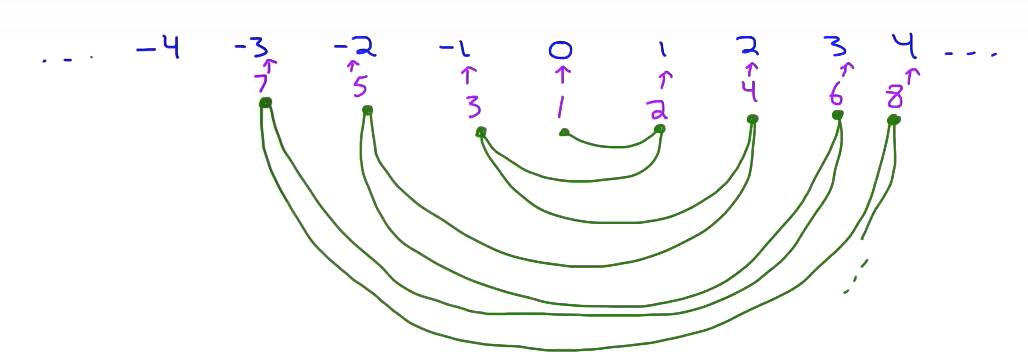
\includegraphics[width=0.5\textwidth]{z_zpos_cardinality}
\end{figure}

The function $f:\mathbb Z^+ \rightarrow \mathbb Z$ defined by $$f(n) = \frac{n}{2}\qquad \text{if $n\in\mathbb Z^+$ is even}$$ $$f(n) = -\frac{n-1}{2}\qquad \text{if $n\in\mathbb Z^+$ is odd}$$ is a bijection.

\subsection{Counting Sets}
\begin{definition}
    A set is called \underline{countably infinite} if and only if it has the same cardinality as the set of positive integers $\mathbb Z^+$
\end{definition}

\begin{example}
    $\mathbb Z$, $2\mathbb Z$, $\mathbb Q^+$, $\mathbb Q$ are all countably infinite.
\end{example}

\begin{definition}
    A set is called \underline{countable} if and only if it is finite or countably infinite. A set that is not countable is called \underline{uncountable}.
\end{definition}
\begin{theorm}
    Any subset of any countable set is countable.
\end{theorm}

Corollary: any set with an uncountable subset is uncountable.

\begin{theorm}
    The set $\left\{x\in\mathbb R | 0 < x < 1\right\}$ is uncountable.
\end{theorm}

Note: every real number between $0$ and $1$ has a unique decimal representation except that $$0.199999\dots = 0.2000\dots$$ and for such numbers, we agree to take the one that ends in all $0$'s.

\begin{proof}
    Suppose the theorem is false.
    Then $\left\{x\in\mathbb R | 0 < x < 1\right\}$ is countable, so the decimal representations of these numbers can be written in a list.
    \begin{equation*}
            \begin{array}{c}
                0.a_{11}a_{12}a_{13}a_{14}\dots a_{1n}\dots \\
                0.a_{21}a_{22}a_{23}a_{24}\dots a_{2n}\dots \\
                0.a_{31}a_{32}a_{33}a_{34}\dots a_{3n}\dots \\
                \vdots
            \end{array}
    \end{equation*}
    We now construct a new decimal number $$d = 0.d_1d_2d_3\dots d_n \dots$$ as follows \begin{equation*}
    \left\{\begin{array}{ll}
        1 & \text{if $a_{nn} \neq 1$} \\
        2 & \text{if $a_{nn} = 1$}
\end{array}\right.
    \end{equation*}

    For instance, take the above $a$ numbers as
    \begin{equation*}
            \begin{array}{c}
                0.120411\dots \\
                0.201377\dots \\
                0.135600\dots \\
                0.897124\dots \\
                \vdots
            \end{array}
    \end{equation*}

    So $$d = 0.2112\dots$$ Note that for each integer $n\in\mathbb Z^+$, $d$ differs from the n\ts{th} real number in the list because it differs in the n\ts{th} decimal place.

    Thus, $d\in\left\{x\in\mathbb R | 0 < x < 1\right\}$ but $d$ does not belong to the list of all real numbers between $0$ and $1$, which is a contradiction.

    Therefore $\left\{x\in\mathbb R | 0 < x < 1\right\}$ is uncountable.
\end{proof}

This shows that since $\left(0,1\right)\subseteq \mathbb R$ and $\left(0,1\right)$ is uncountable, $\mathbb R$ is uncountable.

\subsubsection{Comparing Cardinalities}
\begin{enumerate}
    \item $|X| \leq |Y|$ if and only if $\exists$ injective $f:X\rightarrow Y$
    \item $|X| \geq |Y|$ if and only if $\exists$ surjective $f:X\rightarrow Y$
    \item $|X| < |Y|$ if and only if \begin{enumerate}
        \item $\exists f:X\rightarrow Y$ such that $f$ is injective
        \item $\nexists f:X\rightarrow Y$ such that $f$ is bijective
    \end{enumerate}
    \item $|X| > |Y|$ if and only if \begin{enumerate}
        \item $\exists f:X\rightarrow Y$ such that $f$ is surjective
        \item $\nexists f:X\rightarrow Y$ such that $f$ is bijective
    \end{enumerate}
\end{enumerate}

\begin{definition}
    $|\emptyset| < |X|$ and $|X| > |\emptyset|$ for all $X\neq \emptyset$
\end{definition}

\subsubsection{The Schroder-Bernstein Theorm}
If $|X| \leq |Y|$ and $|X| \geq |Y|$, then $|X| = |Y|$.

Thus, to show $|X| = |Y|$, it is enough to find
\begin{enumerate}
    \item an injective function $X\rightarrow Y$ and
    \item a surjective function $X\rightarrow Y$
\end{enumerate}
OR
\begin{enumerate}
    \item an injective function $X\rightarrow Y$ and
    \item an injective function $Y\rightarrow X$
\end{enumerate}
OR
\begin{enumerate}
    \item a surjective function $X\rightarrow Y$ and
    \item a surjective function $Y\rightarrow X$
\end{enumerate}

This can be much easier than finding a bijection.

\begin{example}
    Show $|\mathbb Z^+| = |\mathbb Q^+|$ using the Schroder-Bernstein theorem.

    \begin{enumerate}
        \item The function $f:\mathbb Z^+ \rightarrow Q^+$ is defined by $f(n) = n\,\forall n\in\mathbb Z^+$ is injective $\therefore |\mathbb Z^+| \leq |\mathbb Q^+|$
        \item Let $g:\mathbb Q^+ \rightarrow \mathbb Z^+$ be defined as follows: for each $q\in\mathbb Q^+$, let $q = \frac{a}{b}$ where $a,b\in\mathbb Z^+$, $b\neq 0$ and $\text{gcd}(a,b)= 1$ and let $g(q) = 2^a 3^b$.
    \end{enumerate}

    Proof that $g$ is injective:

    Let $q_1 = \frac{a}{b}$ and $q_2 = \frac{c}{d}$ as described above and suppose $g(q_1) = g(q_2)$. Then $2^a 3^b = 2^c 3^d$. By unique prime factorisation, $a=c$ and $b=d$. Hence, $q_1=q_2$ so $g$ is injective. $\therefore |\mathbb Q^+| \leq |\mathbb Z^+|$.
\end{example}

\subsection{Relations on Sets}
\begin{definition}
    Given sets $A$ and $B$, a \underline{binary relation} $R$ from $A$ to $B$ is a subset of $A\times B$. If $(x,y)\in\mathbb R$ we also write $xRy$ and say that $x$ is \underline{related} to $y$. Other symbols may be used to denote a relation ($\rho, \sigma, \tau,$ etc)
\end{definition}

\begin{definition}
    If $R$ is a binary relation from $A$ to $B$, the the \underline{inverse relation} $R^{-1}$ is defined from $B$ to $A$ by $$R^{-1} = \left\{(b,a)\in B\times A | (a,b)\in R\right\}$$

    So for all $a\in A$ and $b\in B$, $$(b,a)\in R^{-1} \text{ if and only if }(a,b)\in R$$
\end{definition}
A relation on a set A, is a relation from A to A.\\
\newpage
\begin{definition}
    Let R be a relation on a set A.\\
    \begin{enumerate}
        \item R is reflexive if and only if \(\forall x \in A, ~~xRx\)
        \item R is symmetric if and only if \(\forall x,y \in A\) if \(xRy\) then \(yRx\)
        \item R is transitive if and only if \(\forall x,y,z \in A\) if \(xRy\) and \(yRz\), then \(xRz\)
    \end{enumerate}
\end{definition}
Note that a relation R on a set A is symmetric if and only if \(R = r^{-1}\).\\
\begin{definition}
    R is an equivalence relation if R is symmetric, reflexive and transitive.
\end{definition}
\begin{definition}
    Let R be an equivalence relation on a set A and let \(a \in A\).\\
    The equivalence class of a is \[[a] = \{x\in A | xRa\}\]
    So, \(\forall x\in A\quad x\in [a] \iff xRa\)
\end{definition}
\begin{theorm}
    If R is an equivalence relation on a set A and \(a, b \in A\) satisfy \(aRb\), then \([a] = [b]\).
\end{theorm}
\begin{theorm}
    If R is an equivalence relation on a set A and \(a, b \in A\) and \([a] \cap [b] \neq \emptyset\) then \([a] = [b]\).
\end{theorm}
\begin{theorm}
    If R is an equivalence relation on a set A then the set of equivalence classes of R forms a partition of A. That is, the union of all the classes is A and the intersection of any two distinct classes is empty.\\
    Given a partition of a set A, the binary relation R induced by the partition is defined:\\
    for all \(x, y \in A\), \(xRy \iff\) there is a set in the partition containing both x and y.
\end{theorm}
\begin{theorm}
    Given a partition of a set A, and the binary relation R, induced by the partition, it follows that R is reflexive, symmetric and transitive.
\end{theorm}
\begin{definition}
    A relation R on a set A is antisymmetric if and only if \(\forall a, b \in A\) if \(aRb\) and \(bRa\) then \(a=b\)
\end{definition}
\begin{definition}
    Let R be a relation on a set A. Elements \(a, b\in A\) are comparable if and only if \(aRb\) or \(bRa\). Otherwise, a and b are non-comparable.
\end{definition}
\begin{definition}
    Let R be a relation on a set A. R is a total order relation if and only if, R is a partial order relation such that all elements are comparable.\\
    That is, R is a total order relation if and only if: Reflexive, antisymmetric, transitive and \(\forall a, b \in A\) either \(aRb\) or \(bRa\).
\end{definition}

\section{Groups}
\begin{definition}
    Let $G$ be a set and let $*$ be a binary operation $*:G\to G$. We call $(G, *)$ a \emph{group} if it has the following properties:
    \begin{enumerate}
        \item Closure: for all $g,\,h\in G,\, g*h\in G$
        \item Associative: for all $g,h,k\in G$, $(g*h)*k = g*(h*k)$
        \item Identity: there exists some element $e\in G$ such that $e*g = g*e = g$ $\forall g\in G$
        \item Inverses: for all $g\in G$ there exists some element $g^{-1}\in G$ such that $g*g^{-1} = g^{-1}g = e$
    \end{enumerate}
\end{definition}

\begin{definition}
    For a positive integer $n$, let $\mathbb Z_n$ denote the equivalence classes of integers modulo $n$

    $$\mathbb Z_n = \left\{[0],\,[1],\,[2],\,\dots,\,[n-1]\right\}$$

    Define $+:\mathbb Z_n \times \mathbb Z_n \to \mathbb Z_n$ by $$[a] + [b] = [a+b]$$

    Define $\cdot:\mathbb Z_n \times \mathbb Z_n \to \mathbb Z_n$ by $$[a] \cdot [b] = [a\cdot b]$$
\end{definition}
\begin{definition}
    A group is abelian if the operation \(*\) is commutative. That is,
    \[\forall g, h\in G \qquad g*h = h*g\]
\end{definition}
\begin{theorm}
    Identity element is unique.\\
    Every element in a group has a unique inverse.
\end{theorm}\newpage
\subsection{Subgroup}
\begin{definition}
    Let $(G, *)$ be a group and let $H \subseteq G$. We say that $H$ is a \emph{subgroup} of $G$ if $(H, *)$ is itself a group.

    That is, it is a subgroup of $G$ if
    \begin{enumerate}
        \item for all $g,h\in H$, we have $g*h\in H$ (closure)
        \item if $e$ is the identity for $(G, *)$ then $e\in H$ (identity)
        \item for all $h\in H$, if $h^{-1}$ is the inverse of $h$ in $(G, *)$, then $h^{-1}\in H$ (inverses)
    \end{enumerate}

    We write $H \leq G$ to denote $H$ is a subgroup of $G$, when the context of groups is clear (i.e. not leq).

    If $H\leq G$ and $H \neq G$, we say $H$ is a \underline{proper} subgroup of $G$.

    If $e$ is the identity of group $G$, the \underline{trivial} subgroup of $G$ is $\left\{e\right\}$.
\end{definition}
\begin{definition}
    Given a group \(G, *\) and an element \(g \in G\), we can define the powers of g as follows.\\
    \begin{enumerate}
        \item \(g^k\) denotes \(g*g*\cdots*g\) k times for some \(k\in \mathbb Z^+\)
        \item \(g^{-k}\) denotes \(g^{-1}*g^{-1}*\cdots*g^{-1}\) k times for some \(k\in \mathbb Z^+\)
        \item \(g^0\) denotes the identity element, e.
    \end{enumerate}
\end{definition}
\begin{definition}
    Let \(a\in  G\) be an element of a group \((G, *)\). We let,
        \[\{\langle a \rangle = a^k | k\in \mathbb Z\}\]
        \[\{\cdots, a^{-2}, a^{-1}, e, a^1, a^2, \cdots\}\]
    We call this the set generated by a. \\
    Note that \(\langle a \rangle\) is a subgroup of G and is called the cyclic subgroup. If G has a cyclic subgroup, G is cyclic and that a is the generator of G.
\end{definition}
\begin{definition}
    Two groups \((G, *)\) and \((H, \circ)\) are isomorphic if and only if there exists a bijection \(f: G\to H\) such that forall \(x, y \in G\), \[f(x*y) = f(x)\circ f(y)\]
    Such a bijection is called an isomorphism.\\
    If G and H are isomorphic, then they must have the same properties. (number of elements, abelian, number of subgroups).\\
\end{definition}

\begin{theorm}
    For any prime P, \((\mathbb Z_p - \{0\}, \cdot)\) is isomorphic to \(\mathbb Z_{p-1}, +\).
\end{theorm}
\begin{theorm}
    Suppose \(n,m \in \mathbb Z^+\).\\
    \(\mathbb Z_n \times \mathbb Z_m, +\) is isomorphic to \((\mathbb Z_{nm}, +)\) if and only if \(gcd(n,m) = 1\)
\end{theorm}
\section{Counting}
\begin{example}
    Suppose a restaurant has 5 types of cake and 2 types of ice cream to select for dessert.
    \begin{enumerate}
        \item How many choices for dessert are there if you select one cake and one ice cream?
        There are $5\cdot 2 = 10$ choices. \emph{This is a sequence of tasks - first, choose a dessert, then, choose an ice cream}.
        \item How many choices for dessert are there if you select either one cake or one ice cream, but not both?
        There are $5 + 2 = 7$ choices. \emph{These are two distinct cases}.
    \end{enumerate}
\end{example}

\begin{example}
    Consider a password consisting of 3 letters from the set $\left\{A,\,B,\,C,\,\dots,\,Z\right\}$.
    \begin{enumerate}
        \item How many passwords are possible?
        There are 26 choices for each of the 1st, 2nd and 3rd letters, so there are $$26\cdot 26\cdot 26 = 17576 \text{ possiblities}$$
        \item How many passwords contain no repeated letters?
        There are 26 letters for the 1st letter, 25 for the 2nd and 24 for the 3rd.
        $$\therefore 26\cdot 25\cdot 24 = 15600 \text{ possiblities}$$
        \item How many passwords use only vowels or only consonants?
        $$\text{option } 1 \text{ (only vowels) } + \text{option } 2\text{ (only consonants)}$$
        $$5^3 + 21^3 = 9386$$
    \end{enumerate}
\end{example}

\begin{definition}
    A \underline{permutation} of a set of objects is an arrangement of the objects into an order.
\end{definition}

\begin{example}
    How many permutations of the letters in the word \emph{SWITCH} are there? i.e. SWITCH, CWITHS, etc.

    $$\text{\# of these} = 6\cdot 5\cdot 4\cdot 3\cdot 2\cdot 1 = 6! = 720$$
\end{example}

\begin{theorm}
    For any $n\in\mathbb Z^+$, the number of permutations of a set with $n$ elements is $n!$.
\end{theorm}

\begin{example}
    Consider the permutations of the letters of the word \emph{OBJECTS}. How many permutations start with a vowel?

    Option 1: start with ``o'': $6\cdot 5\cdot 4\cdot 3\cdot 2\cdot 1 = 6!$ \\
    Option 2: start with ``e'': $6\cdot 5\cdot 4\cdot 3\cdot 2\cdot 1 = 6!$
    \\
    Answer: $6!+6! = 1440$.
\end{example}

\begin{example}
    Consider all license plates consisting of 3 digits from the set $\left\{0,\,1,\,\dots,\,9\right\}$ followed by 3 letters from the set $\left\{A,\,B,\,\dots,\,Z\right\}$

    \begin{enumerate}
        \item How many license plates are possible?
        $$10\cdot 10\cdot 10 \cdot 26\cdot 26\cdot 26 = 17576000$$
        \item How many license plates have no repeated symbols?
        $$10\cdot 9\cdot 8\cdot 26\cdot 25\cdot 24 = 11232000$$
        \item How many license plates have at least one repeated symbol?
        We know the total number of license plates and the number of those with no repeated symbols, so the rest must have at least one repeated symbol. $$\therefore 17576000 - 11232000 = 6344000$$
    \end{enumerate}
\end{example}

Let $n$ and $r$ to be non-negative integers.

Problem: \emph{Select $r$ elements from a set containing $n$ elements. How many ways are there to do the selection?}

The answer depends on:
\begin{itemize}
    \item whether or not order matters
    \item whether or not repetition is allowed
\end{itemize}

Case where order matters and repetition is allowed.

\begin{example}
    We have a new ATM card and need to select a PIN. We may choose four digits from the set 
    \[\{0,\,1,\,2,\,3,\,4,\,5,\,6,\,7,\,8,\,9\}\]
    Order matters, and we may repeat. How many PINs are there?

    In each of the four selections we have 10 choices, and hence there are $10^4$ possibilities.
\end{example}

Fact: the number of selections of $r$ elements from a set containing $n$ elements where order matters and repetition is allowed is $n^r$.

Case where order matters, and there is no repetition.

\begin{example}
    If there are 7 runners, how many ways can 1st, 2nd and 3rd be awarded? $$7\cdot 6\cdot 5 = 210$$
\end{example}

\begin{definition}
    Let $n$ and $r$ be non-negative integers with $r\leq n$. An \underline{r-permutation} of a set of $n$ elements is an ordered selection of $r$ elements taken from the set of $n$ elements. The number of r-permutations of a set of $n$ elements is denoted $P(n,r)$ or $nPr$.
\end{definition}

\newpage
\begin{theorm}
    If $n,\,r\in\mathbb Z$ and $1\leq r\leq n$, then $$P(n,\,r) = n(n-1)(n-2)\dots (n-r+1) = \frac{n!}{\left(n-r\right)!}$$
\end{theorm}

Case where order doesn't matter, and repetition is not allowed.

\begin{example}
    In how many ways can $5$ students be selected from a class of $15$ to form a committee?

    If we assume order did matter, we would count as in case 2, to get $$15\cdot 14\cdot 13\cdot 12\cdot 11 = 360360$$

    But order does not matter, and each set of students was counted $5! = 120$ times, so the actual number of choices is $$\frac{360360}{120} = 3003$$
\end{example}

\begin{definition}
    Let $n$ and $r$ be non-negative integers with $r\leq n$. An \underline{r-combination} of a set of $n$ elements is a subset of $r$ of the $n$ elements. The number of $r$-combinations of a set of $n$ elements is denotes $C(n,r)$ or $nCr$ or, more commonly, $\left(^n_r\right)$ which is read ``$n$ choose $r$''.
\end{definition}

\begin{theorm}
    If $n$ and $r$ are non-negative integers and $r\leq n$, then $$\left(^n_r\right) = \frac{P(n,r)}{r!} = \frac{n!}{r!(n-r)!}$$
\end{theorm}

Case where order does not matter, and repetition is allowed.

\begin{example}
    Suppose a store has 4 large buckets, each with a different type of coloured candy: red, blue, yellow, pink. If you must select a total of $7$ candies, how many different choices do you have?

    Select $7$ elements from $\{r,\,b,\,y,\,p\}$ (repetition allowed) where order doesn't matter (i.e. ``rrbbyyy'' is the same as ``ryrybby'')

    Answer = $120$.
\end{example}

\newpage
\begin{example}
    How many permutations of the letters ``ALFALFA'' are there?

    Method (1).
    \begin{itemize}
        \item select positions for the 3 A's
        \item select positions for the 2 F's
        \item put the 2 L's in the remaining positions
    \end{itemize}

    Answer: $$\left(^7_3\right) \cdot \left(^4_2\right) \cdot 1 = 35 \cdot 6 = 210$$ note the $1$ is really $\left(^2_2\right) = 1$


    Method (2). if the letters were distinct, $$A_1 A_2 A_3 F_1 F_2 L_1 L_2$$ there would be $7! = 5040$ possiblities. Now, make the 3 A's indistinguishable. We have counted $$A_1 F_1 F_2 L_2 L_1 A_2 A_3$$ and $$A_2 F_1 F_2 L_2 L_1 A_1 A_3$$ as different solutions, so we have over counted by $3! = 6$ times. Thus, $\frac{5040}{6} = 840$ possible solutions.

    Now make the 2 F's indistinguishable: we have over counted by $2$ times, so we have $\frac{840}{2!} = 420$ possible solutions. Finally, make the 2 L's indistinguishable: we have over counted by $2!$ times, so we have $\frac{420}{2!} = 210$ possible solutions.
\end{example}

\begin{theorm}
    Suppose you have $n$ objects of which $n_1$ are if type $1$, $n_2$ are of type $2$, etc. The number of distinct permutations of the $n$ objects is $$\left(^n_{n_1}\right)\left(^{n-n_1}_{n_2}\right)\left(^{n-n_1-n_2}_{n)3}\right)\dots\left(^{n-n_1-n_2-\dots -n_{k-1}}_{n_k}\right) = \frac{n!}{n_1!n_2!\dots n_k!}$$
\end{theorm}

\subsection{Inclusion and Exclusion}
\begin{example}
    In a fishtank, there are $14$ blue fish, $7$ striped fish, and $4$ fish that are both blue and striped. How many fish are blue or striped?

    If we add the blue fish and the striped fish, we get $14+7=21$. However, we counted the blue striped fish twice (once for being blue, once for being striped), so the actual answer is $(14+7)-4=17$.
\end{example}

\begin{theorm}
    Let $A$ and $B$ be disjoint finite sets, the $|A\cup B| = |A| + |B|$
\end{theorm}

More generally,
\newpage
\begin{theorm}
    For any finite sets $A$ and $B$, $|A\cup B| = |A|+|B| - |A\cap B|$
\end{theorm}

\begin{definition}
    The \underline{Inclusion/Exclusion Principle} (for $2$ or $3$ sets)...

    If $A$, $B$, $C$ are any finite sets, then
    $$|A\cup B| = |A| + |B| - |A\cap B|$$
    and
    $$|A\cup B\cup C| = |A| + |B| + |C| - |A\cap B| - |A\cap C| - |B\cap C| + |A\cap B\cap C|$$
\end{definition}

\subsection{Pigeonhole Principle}
\begin{definition}
    \underline{The Pigeonhole Principle}: Suppose you have $n$ pigeons sitting in $k$ pigeonholes. If $n > k$, then at least one of the pigeonholes contains at least two pigeons.

    \begin{example}
        5 pigeons, 4 holes, at least 1 hole must have more than 1 pigeon.
    \end{example}

    Equivalently, a function from a finite set to a smaller finite set cannot be one-to-one.
\end{definition}

The \underline{contrapositive} of the pigeonhole principle is: Suppose you have $n$ pigeons sitting in $k$ pigeonholes. If each pigeonhole contains at most one pigeon, then $n\leq k$.

\begin{example}
    If you have $3$ different colours in your drawer, what is the minimum number of socks you need to pull out in order to guarantee a matching pair?

    Think of pigeons = socks, pigeonholes = colours. Pull out $4$ socks to guarantee that at least two of them have the same colour.
\end{example}

\begin{example}
    There are $680$ people in a list. Must there be at least two people on the list with the same first and last initials? Explain.

    pigeons = people, pigeonholes = initials.

    There are $26\cdot 26 = 676$ possible options for first and last initials. Since $680 > 676$, the pigeonhole principle implies at least 2 people must have the same initials.
\end{example}
\newpage
\begin{definition}
    \underline{The generalised pigeonhole principle}

    Suppose you have $n$ pigeons sitting in $k$ pigeonholes. If $n>k\cdot m$, then at least one of the pigeonholes contains at least $m+1$ pigeons.

    Contrapositive: suppose you have $n$ pigeons sitting in $k$ pigeonholes. If each pigeonhole contains at most $m$ pigeons, then $n\leq km$.
\end{definition}

\begin{example}
    Show that in a group of $25$ people, at least $3$ must be born in the same month.

    Let $n=25$ and $m=2$.

    We have $25$ pigeons (people) and $12$ pigeonholes (months).

    Since $n > 12\cdot 2$, the generalised pigeonhole principle implies that there is a month which $\geq 3$ people from the group have a birthday.
\end{example}

\section{Graph Theory}
Before we begin with formal definitions, let us start with an example. Suppose we have a group of people and some of them are friends. We may represent these by drawing a point for each person, and a line for each friendship. Obviously, the position of the dots and lines does \emph{not} matter, just the connections.

\begin{definition}
    A \emph{graph} $G$ consists of two finite sets:
    \begin{itemize}
        \item a non-empty set $V(G)$ of vertices, and
        \item a (possibly empty) set $E(G)$ of edges, where each edge is associated with a set $\left\{v,w\right\}\subseteq V(G)$
    \end{itemize}

    The vertices $v$ and $w$ are called the end points of the edge.
\end{definition}

\begin{example}
    \begin{figure}[H]
        \centering
        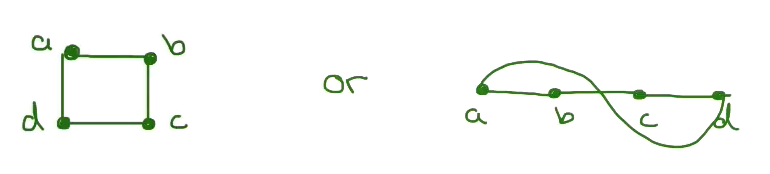
\includegraphics[width=0.5\textwidth]{basic_graph}
    \end{figure}

    This graph $G$ has $V(G) = \left\{a,\,b,\,c,\,d\right\}$ and has $4$ edges whose endpoints are $$\left\{a,\,b\right\},\,\left\{b,\,c\right\},\,\left\{c,\,d\right\},\,\left\{a,\,d\right\}$$
\end{example}

\begin{definition}
    A \underline{loop} is an edge whose endpoints are equal, which is denoted $\{v,\,v\}$ or $\{v\}$
\end{definition}

\begin{definition}
    \underline{Parallel edges} (or \underline{multiple edges}) are two or more edges with the same set of endpoints.
\end{definition}

\begin{definition}
    A \underline{simple graph} is a graph with no loops or parallel edges.

    \begin{figure}[H]
        \centering
        
\includegraphics[width=0.5\textwidth]{simplicity}
    \end{figure}
\end{definition}
\newpage
\begin{example}
    Referred to below.
    \begin{figure}[H]
        \centering
        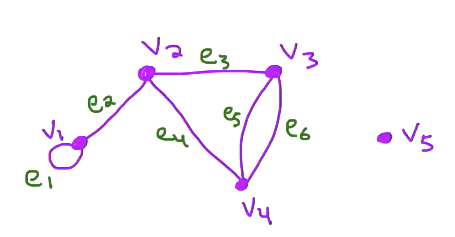
\includegraphics[width=0.5\textwidth]{example_graph_for_defs}
    \end{figure}
\end{example}

\begin{definition}
    An edge and a vertex are \underline{incident} if and only if the vertex is an endpoint of the edge.
    \\ \\
    Ex. $e_3$ is incident with $v_2$ and $v_3$. $v_1$ is incident with $e_1$ and $e_2$.
\end{definition}

\begin{definition}
    Two edges are \underline{adjacent} if they are incident with the same vertex.

    The vertices are \underline{adjacent} if they are connected by an edge (ie there is an edge they are both incident with).
    \\ \\
    Ex. $e_2$ and $e_3$ are adjacent. $v_2$ and $v_4$ are adjacent. $v_1$ and $v_4$ are non-adjacent.
\end{definition}

\begin{definition}
    An \underline{isolated} vertex is a vertex which is incident with no edges. Namely, $v_5$ above.
\end{definition}

\begin{definition}
    The \underline{degree} of a vertex $v$ is the number of edges incident with $v$, where we count each loop \emph{twice}. We write this as $\text{deg}(v)$.
\end{definition}

\begin{theorm}
    \underline{The Handshake Theorm}

    Let $G$ be a graph with $n$ vertices $$V(G) = \left\{v_1,\,v_2,\,v_3,\,\dots,\,v_n\right\}$$

    Then $$\sum_{i=1}^n \text{deg}(v_i) = \text{deg}(v_1) + \text{deg}(v_2) + \dots + \text{deg}(v_n) = 2 \cdot |E(G)|$$
\end{theorm}

\subsection{Getting Between Vertices}
Let $G$ be graph and let $v$ and $w$ be vertices in $G$. A \emph{walk} from $v$ to $w$ is a finite alternating sequence 
\begin{equation}
    v_0 e_1 v_1 e_2 \dots v_{n-1}e_n v_n
\end{equation}

of vertices and edges where $v_0 = v$, $v_n = w$, and $e_i$ is an edge with endpoints $\left\{v_{i-1},\,v_i\right\}$ for $i\in\left\{1,\,\dots,\,n\right\}$

\begin{example}
    \begin{figure}[H]
        \centering
        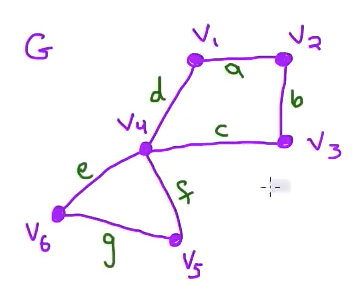
\includegraphics[width=0.25\textwidth]{walk}
    \end{figure}
    $v_5 f v_4 c v_3 c v_4 e v_6$ is a walk from $v_5$ to $v_6$.

    Also, $v_5 g v_6$ is a walk from $v_5$ to $v_6$.
\end{example}

\begin{definition}
    A graph $G$ is \underline{connected} if and only if, given any two vertices $v$ and $w$ in $G$, there is a walk from $v$ to $w$.

    A \underline{trail} is a walk whose edges are distinct.

    A \underline{circuit} is a trail that starts and ends at the same vertex.
\end{definition}

\begin{definition}
    Let $G$ be a graph. An \underline{Euler circuit} for $G$ is a circuit that contains every edge of $G$ exactly once.

    Lemma: if a graph $G$ has an Euler circuit, then each vertex has even degree. Proof in lec 35.
\end{definition}

\begin{theorm}
    Let $G$ be a connected graph. Then $G$ has an Euler circuit if and only if every vertex of $G$ has even degree.
\end{theorm}

\begin{definition}
    Let $G$ be a graph and let $u,\, v \in V(G)$. An \underline{Euler trail} from $u$ to $v$ is a trail from $u$ to $v$ that uses every edge exactly once.
\end{definition}
\begin{theorm}
    Let G be a connected graph and let \(u, v\in v(G)\).\\
    If \(u = v\) then G has an Euler trail from u to v if and only if every vertex of G has even degree.\\
    If \(u \neq v\) then G has an Euler trail from u to v iff u and v have odd degree and all other vertices have even degree.
\end{theorm}



\end{document}

